\documentclass{TDP003mall}

\newcommand{\version}{Version 0.6}
\author{IP1 2022}
\title{Installationsmanual\\för\\ Portföljsystem}
\date{2022-09-16}
\rhead{IP1 2022}

\usepackage{subcaption}
\usepackage{float}
\usepackage{graphicx}
\graphicspath{ {./images/} }

\begin{document}
\projectpage
\section*{Revisionshistorik}
\begin{table}[!h]
\begin{tabularx}{\linewidth}{|l|X|l|}
\hline
Ver. & Revisionsbeskrivning & Datum \\\hline
0.1 & Grundstruktur av dokument samt introduktion skapat & 16/9 \\\hline
0.2 & Installation av git & 16/9 \\\hline
0.3 & Installation av Flask och Jinja2 & 16/9 \\\hline
0.4 & Lade till beskrivning av Gitlab, Python3 och Emacs & 16/9 \\\hline
0.5 & Lade till beskrivning LaTeX & 19/9 \\\hline
0.5 & Tog bort dublett av stycket "Virtuell miljö" & 19/9 \\\hline
0.6 & Lade till extra beskrivning av LaTeX, uppdaterade versionen för dokumentet & 20/9\\\hline
0.7 & Kontroll av installation Emacs & 21/9\\\hline
0.8 & Hantering och navigering av terminalen & 22/9\\\hline
0.9 & Installationshandledning för andra distributioner än Ubuntu & 22/9\\\hline
\end{tabularx}
\end{table}


\section*{Introduktion}
Denna manual förklarar installation av en utvecklingsmiljö som kan hantera skapandet, underhållandet etcetera avseende
en portfolio som dokumenterar gjorda projekt. Portfolion implementeras som en webbplats.\\
Manualen bistår med en väl förklarande handledning när det kommer till att installera de program och paket som behövs
samt uppsättande och hantering av en projektkatalog samt virtuell miljö.\\\\ I denna manual ges specifika instruktioner för installation på Debian-baserade distributioner (såsom Ubuntu eller Linux Mint), Fedora samt Arch och distributioner baserade på Arch (exempelvis Endeavour OS). Motsvarande kommandon för att installera programvaran på övriga distributioner (exempelvis openSUSE) tillhandahåller inte denna installationsmanual.\\\\
Första delen behandlar installation av essentiella program och paket. Andra delen hanterar skapandet av en projektkatalog
samt implementering av versionshantering, git. Sista delen behandlar implementerande av en virtuell miljö.

\section*{Hantering och navigering av terminalen}
Installationsmanualen listar en rad installationskommandon nedan du kommer använda i terminalen. Du kommer därför behöva följande grundläggande koll på hur du öppnar och hanterar terminalen för installation av dessa program.

\subsubsection*{Öppna terminalen}
Terminalen når du genom att antingen söka i applikationsmenyn: ``terminal''

Eller genom kortkommandot ctrl + t.

\subsubsection*{Se nuvarande arbetskatalog}
Vid hantering av git och den virtuella miljön kommer det vara viktigt att du vet vilken katalog du står i just nu.
Kommandot för ``working directory'' är därför relevant. För att see din nuvarnade arbetskatalog, skriv i terminalen:

>> wkdir

\subsubsection*{Byt katalaog}
Kommandot cd ``change directory'' används för förflyttning av din nuvarande arbetskatalog. I terminalen skrivs följande:

>> cd katalognamn/

Där ``katalognamn/'' hänvisar vilken katalog du vill navigera till.

Behöver du navigera tillbaka till en yttre katalog i katalogträdet används följande kommando:

>> cd ..

\subsubsection*{Lista katalog}
Önskar du visa innehållet i din nuvarande katalog kan du använda terminalkommandot ls ``list files''. Detta skrivs in i
terminalen som följande:

>> ls

\section*{Program- samt paketinstallation}

\subsection{Python3}
Python är ett programmeringsspråk som är förinstallerat på Ubuntu-distributioner. Versionen som är installerad är Python 3.
\subsection{Installation av text editor}

Det finns ett antal text editors som är gratis att använda. De mest populära är bland annat Visual Studio Code, Emacs och Pycharm.
Installationen av dessa editor kan kräva det senaste versionen av Linux. För att upgradera till den senaste versionen av behöver följade kommando skrivas, beroende på distribution:

\textbf{Ubuntu / Linux Mint:}\\
sudo apt update\\
sudo apt upgrade

\textbf{Fedora:}\\
sudo dnf upgrade --refresh

\textbf{Arch:}\\
sudo pacman -Syu

\subsubsection*{Emacs}

Emacs är en textredigerare och för att installera textredigeraren på skrivs följande kommando:

\textbf{Ubuntu / Linux Mint:}\\
sudo apt install emacs

\textbf{Fedora:}\\
sudo dnf install emacs

\textbf{Arch:}\\
sudo pacman -S emacs

För att kontrollera att emacs har installerats används detta kommando:

\textbf{emacs --version}\\

\textbf{Kontroll av installation}
\begin{figure}[H]
        \centering
        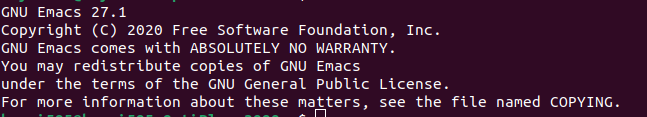
\includegraphics[width=0.8\textwidth]{images/emacs kontroll.png}
        \caption{Resultat av "emacs --version"}
\end{figure}
\subsubsection*{Visual Studio Code}

Visual Studio Code är en text editor som är skapad och underhålls av Microsoft för Windows, Linux och macOS, och finns tillgängligt på vissa distributioners repostories. Vissa distributioner (exempelvis Arch) har en Open Source-variant av Visual Studio Code vid namn Code - OSS, som funktionellt sett är samma program som även tillhandahålls av Microsoft.

Vilken version som passar bäst skiljer sig mellan distributioner. Men generellt är det enklast att installera programmet genom Snap, som finns förinstallerat på Ubuntu och andra användarvänliga distributioner.

\textbf{Snap-installation (för exempelvis Ubuntu):}\\
sudo snap install --classic code

\textbf{Fedora:}\\
Visual Studio Code finns inte i Fedoras egna repositories, rekommendationen är därför att installera programmet via Flatpak.\\
sudo dnf install flatpak -y\\
sudo flatpak remote-add --if-not-exists flathub https://flathub.org/repo/flathub.flatpakrepo\\
flatpak install https://flathub.org/repo/appstream/com.visualstudio.code.flatpakref

\textbf{Arch:}
sudo pacman -S code

\textbf{Programmet kan sedan startas med föjande kommando:}
code

\subsubsection*{PyCharm}

PyCharm är en Integrated Development Environment (IDE). Det finns två versioner: en version som kostar (Professional) och en kostnadsfri (Community). Den här installationsguide använder PyCharm Community.
För att installera PyCharm skrivs följande kommando:

\textbf{Snap-installation (för exempelvis Ubuntu):}\\
sudo snap install pycharm-community -{}-classic

\textbf{Fedora:}\\
PyCharm finns inte i Fedoras egna repositories, rekommendationen är därför att installera programmet via Flatpak.\\
sudo dnf install flatpak -y\\
sudo flatpak remote-add --if-not-exists flathub https://flathub.org/repo/flathub.flatpakrepo\\
flatpak install flathub com.jetbrains.PyCharm-Community

\textbf{Arch (eller andra Arch-baserade distributioner:)}\\
sudo pacman -S pycharm-community-edition

Efter slutförd installation kan följande komando starta PyCharm:

\textbf{pycharm-community}

\subsection*{Git \& Gitlab}
Git är ett versionshanteringssystem som används för att skapa projekt antingen själv eller i grupp.
Det första som behövs göra är att skapa ett projekt på githemsidan och sedan länka en fil till det projektet.
Instruktioner för att länka en fil till gitprojektet finns på startsidan av ditt projekt. Efter en fil är länkad kan
filen som finns i den länkade mappen laddas upp till sitt projekt. Dessa filer kommer att sparas på projektsidan
och om filerna redigeras går det att laddad upp filen igen och då kommer ändringen att sparas som en''commit'' i Git. Alla commits sparas och så det går alltid gå tillbaka till en föregående commit om något har blivit fel.\\\\
För att installera git, kör följande kommandon:\\

\textbf{Ubuntu / Linux Mint:}\\
{sudo apt-get install git-all

\textbf{Fedora:}\\
sudo dnf install git

\textbf{Arch:)}\\
sudo pacman -S git

Kontroll att git har blivit installerat kan kontrolleras genom att skriva git --version i terminalen.

Gitlab är en samarbetsplattform för utveckling. Som namnet antyder så har hemsidan stöd för versionkontroll baserat på Git och har ett web baserat grafisk gränsnitt.  

Innan gitlab kan användas måste en ssh-nyckel som finns på din dator registeras på gitlab. Ssh-keygen används för att skapa säkra shell-sessioner mellan fjärrdatorer över osäkra nätverk genom använding av olika kryptografiska tekniker.

I ".ssh" mappen på den aktuella linux datorn kan ssh-nyckeln skapas med kommandot:

\textbf{ssh-keygen -t rsa -C ''GitLab'' -b 4096}

Sedan bestämms om nyckeln ska ha ett lösenord kopplat till sig, om lösenordet inte är nödvändigt tryck på enter. Sedan kopieras den publika nyckel, d.v.s. ''id\_rsa.pub'' (inte ''id\_rsa.txt'' då det är den privata nyckel), och går in på Gitlab -> Preferences (klickar på profilbilden uppe i högra hörnet) -> SSH Keys och sedan klistrar in nyckeln i textrutan "Key". Därefter ska nyckeln namnges med valfritt namn och trycka på knappen " Add key".

För att börja arbeta med Git så öppna den aktuella katalog som arbetet ska utföras i och skriver kommandot:

\textbf{git init}

För att bidra till ett repo behövs identifiering av vem som skapat en commit via ens användarnamn och e-post. Dessa två saker går att konfigurera i ens Gitkonfiguration med följande kommandon:

\textbf{git config --global user.name " ange namn här"}
\\
\textbf{git config --global user.email " ange e-post här"}

För att hämta filer från ett projekt som finns på GitLab så måste en remote läggas till i den katalog filen ska hämtas till. Det här görs genom att först gå till GitLab-projektet, trycka på "Clone" och kopiera den länk som står under "Clone with SSH". Därefter skriv följande kommandon i den katalog som arbetas i:

\textbf{git remote add origin "SSH-nyckeln här"}

En viktig sak att tänka på när ett jobb mot ett projekt på gitlab utförs är att den lokala versionen och versionen på gitlab är den samma för att undvika konflikter. Innan atbetet börjar är det en bra idé att säkerställa detta, vilket görs med kommandot:

\textbf{git pull}

Det som händer är att om den lokala versionen ligger efter jämfört med gitlabs version kommer gitlabs version att hämtas och slås ihop med den lokala version och det går nu att jobba med den senaste versionen av projektet.\\
För att ladda upp filer som redigerats eller lagts till i efterhand till ett git projekt används följande kommandon:\\\\
\textbf{git add <filnamn>}\\
\textbf{git commit}\\
\textbf{git push}\\

För att undersöka vilka filer som har ändrats så kan det här kommandot användas:

\textbf{git status}

Då jämförs den lokala katalogen mot gitlabs verision och skriver ut alla lokala filers namn som har ändrats i röd färg.

\subsection{Flask och Jinja2}

Flask är ett webbramverk skrivet i python som förenklar utveckligen av webbsidor. Flask använder webbmallssystem för att underlätta utformningen av hemsidor, och som standard används Jinja2.  För att installera Flask (och Jinja2 som medföljer) så behövs en virtuell pythonmiljö. Detta är för att pythonprojekt ofta kräver, eller fungerar bäst, i specifika projektmiljöer. För att skapa en virtuell miljö så behöver det först installeras, vilket görs med kommandot:

\textbf{Ubuntu / Linux Mint}\\
sudo apt install python3.10-venv

\textbf{Fedora:}\\
sudo yum install python-virtualenv

\textbf{Arch:}\\
sudo pacman -S python-virtualenv

Efter det så behöver en virtuell miljö i projektmapp skapas, och det görs genom att stå i mappen i terminalen och skriva:

\textbf{python3 -m venv <namn>}

Namnet här är det namn på miljön som ska skapas, så t.ex. ger 'python3 -m venv venv' en virtuell miljö som heter venv. När den virtuella miljön skapats så behöver den också aktiveras, och det görs genom att stå i samma projektmappen som den skapade miljön och skriva:

\textbf{. /<namn>/bin/activate}

Om allt har gått bra så kommer nu namnet på din virtuella miljö synas först i terminalen. Om den virtuella miljön ska avslutas skrivs 'deactivate' i terminalen. Om pip är installerat går det nu att installera Flask, ifall pip ej är installerat går det att göra med kommandot:

\textbf{sudo apt install python3-pip}

Slutligen kan Flask installeras med kommandot:

\textbf{pip install Flask}

Kommandot installerar inte bara Flask utan också Jinja2, MarkupSafe, Werkzeug, Click och itsdangerous. Om installationen har fungerat så kommer det på sista raden att stå Successfully installed... och sedan alla programmen som installerades.

\subsection*{LaTeX}
För dokumentationen i projektet används LaTeX för att skapa PDF:er. LaTeX är ett 'document preparation system' som fungerar lite olikt andra ordbehandlare såsom exempelvis Microsoft Office som fungerar enligt principen 'What You See Is What You Get'. LaTeX följer istället en princip där författaren fokuserar på innehållet istället för utseendet enligt principen 'What You See Is What You Mean'. LaTeX fungerar likt ett programmeringsspråk genom att en kod skrivs för att bygga upp sitt dokument och sedan kompileras källkoden till ett dokument. Detta innebär att versionshantering blir mycket lättare då hela dokumentet består av text så det går enkelt att se och lösa eventuella konflikter då flera personer jobbar i samma dokument.

Det finns flera olika paket för att installera LaTeX i ubuntu men det enklaste för att slippa ta reda på vilka olika paket som behövs är att installera LaTeX med alla tillhörande paket. Detta görs med hjälp av kommandot:

\textbf{sudo apt-get install texlive-full latexmk}

För att kompilera LaTeX-filer, det vill säga filer med filändelsen .tex, så används detta kommando i samma mapp som filen ligger:

\textbf{latexmk -xelatex -pvc filnamn.tex}

Detta genererar en PDF-fil av LaTeX-filen, och gör det möjligt att direkt kunna se förändringar i latex-filen när efter den har redigerats och blivit sparad. Efter att kommandot har körts så går det att fortsätta med att redigera LaTeX-filen, och varje gång filen sparas så komplileras filen automatiskt.

\subsection*{LaTeX Workshop (VScode extension)}
För att underlätta dokument skrivandet med t.ex autocomplete och språkfel korrigering kan LaTeX workshop användas. 
För att installera LaTeX workshop så tas ''extensions'' fram med Ctrl+Shift+X. 
I extensions så är det bara att söka fram LaTeX workshop och installera (specifikt av James Yu).\\

LaTex workshop kommer inte fungera direkt för att LaTeX workshop försöker kompilera med ''pdflatex x 2''. Då latexmk används så är det bara att ändra ordningen på build recepten i settings.json filen. Hittas under \mbox{\textbackslash{Code}\textbackslash{user}\textbackslash{settings.json}\nolinebreak}.
Det är bara att byta plats på ''pdflatex*2'' och ''latexmk(xelatex)''(Se \ref{fig:settingJson}).
\begin{figure}[H]
    \begin{subfigure}{.5\textwidth}
        \centering
        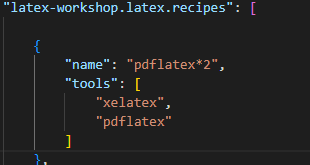
\includegraphics[width=0.8\textwidth]{images/settings0.png}
        \caption{Hur settings.json ser ut först}
    \end{subfigure}
    \begin{subfigure}{.5\textwidth}
        \centering
        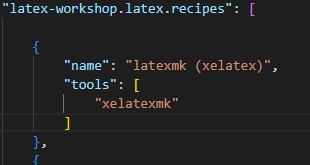
\includegraphics[width=0.8\textwidth]{images/settings1.png}
        \caption{Hur settings.json bör se ut}
    \end{subfigure}
    \caption{Det i settings.json filen som ska bytas ut (allting mellan klammerparenteserna)}
    \label{fig:settingJson}
\end{figure}
Nu går det att kompilera .tex filen, först så ska VScode öppnas med filen: \\\\
\textbf{code dokument.tex}\\\\
För att kompilera använd snabbkommandot Ctrl + Alt + B (eller tryck på den gröna kör knappen längst upp till höger).
Alternativs så kan pdf filen tas fram och uppdateras i ''realtid'' genom att ta fram LaTeX tabben med Ctrl + Alt + X och trycka på ''View LaTeX PDF''.


\section*{Projektkatalog samt git}



\end{document}
